\PassOptionsToPackage{unicode=true}{hyperref} % options for packages loaded elsewhere
\PassOptionsToPackage{hyphens}{url}
\PassOptionsToPackage{dvipsnames,svgnames*,x11names*}{xcolor}
%
\documentclass[12pt,]{article}
\usepackage{lmodern}
\usepackage{setspace}
\setstretch{1.5}
\usepackage{amssymb,amsmath}
\usepackage{ifxetex,ifluatex}
\usepackage{fixltx2e} % provides \textsubscript
\ifnum 0\ifxetex 1\fi\ifluatex 1\fi=0 % if pdftex
  \usepackage[T1]{fontenc}
  \usepackage[utf8]{inputenc}
  \usepackage{textcomp} % provides euro and other symbols
\else % if luatex or xelatex
  \usepackage{unicode-math}
  \defaultfontfeatures{Ligatures=TeX,Scale=MatchLowercase}
    \setmainfont[]{Georgia}
\fi
% use upquote if available, for straight quotes in verbatim environments
\IfFileExists{upquote.sty}{\usepackage{upquote}}{}
% use microtype if available
\IfFileExists{microtype.sty}{%
\usepackage[]{microtype}
\UseMicrotypeSet[protrusion]{basicmath} % disable protrusion for tt fonts
}{}
\IfFileExists{parskip.sty}{%
\usepackage{parskip}
}{% else
\setlength{\parindent}{0pt}
\setlength{\parskip}{6pt plus 2pt minus 1pt}
}
\usepackage{xcolor}
\usepackage{hyperref}
\hypersetup{
            colorlinks=true,
            linkcolor=Maroon,
            citecolor=Blue,
            urlcolor=blue,
            breaklinks=true}
\urlstyle{same}  % don't use monospace font for urls
\usepackage[margin=1.0in]{geometry}
\usepackage{graphicx,grffile}
\makeatletter
\def\maxwidth{\ifdim\Gin@nat@width>\linewidth\linewidth\else\Gin@nat@width\fi}
\def\maxheight{\ifdim\Gin@nat@height>\textheight\textheight\else\Gin@nat@height\fi}
\makeatother
% Scale images if necessary, so that they will not overflow the page
% margins by default, and it is still possible to overwrite the defaults
% using explicit options in \includegraphics[width, height, ...]{}
\setkeys{Gin}{width=\maxwidth,height=\maxheight,keepaspectratio}
\setlength{\emergencystretch}{3em}  % prevent overfull lines
\providecommand{\tightlist}{%
  \setlength{\itemsep}{0pt}\setlength{\parskip}{0pt}}
\setcounter{secnumdepth}{5}

% set default figure placement to htbp
\makeatletter
\def\fps@figure{htbp}
\makeatother

\usepackage[left]{lineno}
\linenumbers
\usepackage{longtable}
\usepackage{graphicx}
\usepackage{booktabs}
\usepackage{listings}
\usepackage{textcomp}
\usepackage{xcolor}
\usepackage{multirow}
\usepackage{subcaption}
\definecolor{listcomment}{rgb}{0.0,0.5,0.0}
\definecolor{listkeyword}{rgb}{0.0,0.0,0.5}
\definecolor{listnumbers}{gray}{0.65}
\definecolor{listlightgray}{gray}{0.955}
\definecolor{listwhite}{gray}{1.0}

\author{}
\date{\vspace{-2.5em}}

\begin{document}

\pagenumbering{gobble}

\setstretch{1}

\begin{centering}

$ $

\vspace{4.cm}

\LARGE

{\bf ANTsX:  A dynamic ecosystem for quantitative biological and medical imaging}

\vspace{0.5 cm}

\normalsize

Nicholas J. Tustison$^{1,9}$,
Philip A. Cook$^{2}$,
Andrew J. Holbrook$^{3}$,
Hans J. Johnson$^{4}$,
John Muschelli$^{5}$,
Gabriel A. Devenyi$^{6}$,
Jeffrey T. Duda$^{2}$,
Sandhitsu R. Das$^{2}$,
Nicholas C. Cullen$^{7}$,
Daniel L. Gillen$^{8}$,
Michael A. Yassa$^{9}$,
James R. Stone$^{1}$,
James C. Gee$^{2}$,
Brian B. Avants$^{1}$
for the Alzheimer’s Disease Neuroimaging Initiative

\footnotesize

$^{1}$Department of Radiology and Medical Imaging, University of Virginia, Charlottesville, VA \\
$^{2}$Department of Radiology, University of Pennsylvania, Philadelphia, PA \\
$^{3}$Department of Biostatistics, University of California, Los Angeles, CA \\
$^{4}$Department of Electrical and Computer Engineering, University of Iowa, Philadelphia, PA \\
$^{5}$School of Public Health, Johns Hopkins University, Baltimore, MD \\
$^{6}$Douglas Mental Health University Institute, Department of Psychiatry, McGill University, Montreal, QC \\
$^{7}$Lund University, Scania, SE \\
$^{8}$Department of Statistics, University of California, Irvine, CA \\
$^{9}$Department of Neurobiology and Behavior, University of California, Irvine, CA \\

\end{centering}

\vspace{4.5 cm}

\scriptsize

Corresponding author:\\
Nicholas J. Tustison, DSc\\
Department of Radiology and Medical Imaging\\
University of Virginia\\
\href{mailto:ntustison@virginia.edu}{\nolinkurl{ntustison@virginia.edu}}

\normalsize

\newpage

\setstretch{1.5}

\hypertarget{abstract}{%
\section*{Abstract}\label{abstract}}
\addcontentsline{toc}{section}{Abstract}

The Advanced Normalizations Tools ecosystem, known as ANTsX, consists of
multiple open-source software libraries which house top-performing
algorithms used worldwide by scientific and research communities for
processing and analyzing biological and medical imaging data. The base
software library, ANTs, is built upon, and contributes to, the
NIH-sponsored Insight Toolkit. Founded in 2008 with the highly regarded
Symmetric Normalization image registration framework, the ANTs library
has since grown to include additional functionality. Recent enhancements
include statistical, visualization, and deep learning capabilities
through interfacing with both the R statistical project (ANTsR) and
Python (ANTsPy). Additionally, the corresponding deep learning
extensions ANTsRNet and ANTsPyNet (built on the popular TensorFlow/Keras
libraries) contain several popular network architectures and trained
models for specific applications. One such comprehensive application is
a deep learning analog for generating cortical thickness data from
structural T1-weighted brain MRI,
\textcolor{blue}{both cross-sectionally and longitudinally}. These
pipelines significantly improve computational efficiency and provide
comparable-to-superior accuracy
\textcolor{blue}{over multiple criteria relative
to} the existing ANTs \textcolor{blue}{workflows} and
\textcolor{blue}{simultaneously} illustrate the importance of the
comprehensive ANTsX approach as a framework for medical image analysis.

\newpage

\hypertarget{the-antsx-ecosystem-a-brief-overview}{%
\section*{The ANTsX ecosystem: A brief
overview}\label{the-antsx-ecosystem-a-brief-overview}}
\addcontentsline{toc}{section}{The ANTsX ecosystem: A brief overview}

\hypertarget{image-registration-origins}{%
\subsection*{Image registration
origins}\label{image-registration-origins}}
\addcontentsline{toc}{subsection}{Image registration origins}

The Advanced Normalization Tools (ANTs) is a state-of-the-art,
open-source software toolkit for image registration, segmentation, and
other functionality for comprehensive biological and medical image
analysis. Historically, ANTs is rooted in advanced image registration
techniques which have been at the forefront of the field due to seminal
contributions that date back to the original elastic matching method of
Bajcsy and co-investigators\textsuperscript{1--3}. Various independent
platforms have been used to evaluate ANTs tools since their early
development. In a landmark paper\textsuperscript{4}, the authors
reported an extensive evaluation using multiple neuroimaging datasets
analyzed by fourteen different registration tools, including the
Symmetric Normalization (SyN) algorithm\textsuperscript{5}, and found
that ``ART, SyN, IRTK, and SPM's DARTEL Toolbox gave the best results
according to overlap and distance measures, with ART and SyN delivering
the most consistently high accuracy across subjects and label sets.''
\textcolor{blue}{Participation in other independent competitions}\textsuperscript{6,7}
\textcolor{blue}{provided additional evidence of
the utility of ANTs registration and other tools.  Despite the extremely
significant potential of deep learning for image registration algorithmic
development}\textsuperscript{8},
\textcolor{blue}{ANTs registration tools
continue to find application in the various biomedical imaging research
communities.}

\hypertarget{current-developments}{%
\subsection*{Current developments}\label{current-developments}}
\addcontentsline{toc}{subsection}{Current developments}

\begin{figure}[htbp]
  \centering
    \includegraphics[width=0.9\textwidth]{Figures/coreANtsXNetTools.png}
    \caption{An illustration of the tools and applications available as part of the
    ANTsRNet and ANTsPyNet deep learning toolkits.  Both libraries take advantage
    of ANTs functionality through their respective language interfaces---ANTsR (R)
    and ANTsPy (Python).  Building on the Keras/TensorFlow language, both libraries
    standardize popular network architectures within the ANTs ecosystem and are
    cross-compatible.  These networks are used to train models and weights for such
    applications as brain extraction which are then disseminated to the public.}
 \label{fig:antsXnetTools}
 \end{figure}

Since its inception, though, ANTs has expanded significantly beyond its
image registration origins. Other core contributions include template
building\textsuperscript{9}, segmentation\textsuperscript{10}, image
preprocessing (e.g., bias correction\textsuperscript{11} and
denoising\textsuperscript{12}), joint label
fusion\textsuperscript{13,14}, and brain cortical thickness
estimation\textsuperscript{15,16} (cf Table \ref{table:papers}).
Additionally, ANTs has been integrated into multiple, publicly available
workflows such as fMRIprep\textsuperscript{17} and the Spinal Cord
Toolbox\textsuperscript{18}. Frequently used ANTs pipelines, such as
cortical thickness estimation\textsuperscript{16}, have been integrated
into Docker containers and packaged as Brain Imaging Data Structure
(BIDS)\textsuperscript{19} and FlyWheel applications (i.e., ``gears'').
It has also been independently ported for various platforms including
Neurodebian\textsuperscript{20} (Debian OS),
Neuroconductor\textsuperscript{21} (the R statistical project), and
Nipype\textsuperscript{22} (Python).
\textcolor{blue}{Additionally, other widely
used software}, such as FreeSurfer\textsuperscript{23}, have
incorporated well-performing and complementary ANTs
components\textsuperscript{11,12} into their own libraries.
\textcolor{blue}{Finally, according to GitHub, recent
unique “clones” have averaged 34 per day with the total number of clones being
approximately twice that many.  50 unique contributors to the ANTs library have
made a total of over 4500 commits. Additional insights into usage can be viewed
at the ANTs GitHub website.}


% Citations of main tools (January 3)
% ANTs registration SyN \cite{Avants:2008aa} = 1057
% ANTs registration (main) \cite{Avants:2011ab} = 535
% template building \cite{Avants:2010aa} = 158

% N4ITK \cite{Tustison:2010ac} = 431
% Atropos \cite{Avants:2011aa} = 106
% KK Cortical thickness (Das) \cite{Das:2009aa} = 80
% KK Cortical thickness (Tustison) \cite{Tustison:2014ab} = 57


\begin{table}
  \small
   \centering
   \vspace{-0.25cm}
   \begin{tabular*}{0.75\textwidth}{l @{\extracolsep{\fill}} c}
    \toprule
    {\bf Functionality} & {\bf Citations}\\
    \cmidrule[1pt](lr){1-2}
    {SyN registration \cite{Avants:2008aa}} & 2314        \\
    bias field correction \cite{Tustison:2010ac} & 1803  \\
    ANTs registration evaluation \cite{Avants:2011ab} & 1736  \\
    joint label fusion   \cite{Wang:2013ab} & 622       \\
    template generation \cite{Avants:2010aa} & 384      \\
    cortical thickness: implementation \cite{Tustison:2014ab} & 262 \\
    ITK integration \cite{Avants:2014aa} & 204           \\
    MAP-MRF segmentation \cite{Avants:2011aa} & 283     \\
    cortical thickness: theory \cite{Das:2009aa} & 156   \\
    \bottomrule
   \end{tabular*}
 \caption{\textcolor{red}{Need to update closer to submission time.}The significance of core ANTs tools in terms of their number of citations (from April 27, 2020).}
 \label{table:papers}
\end{table}


Over the course of its development, ANTs has been extended to
complementary frameworks resulting in the Python- and R-based ANTsPy and
ANTsR toolkits, respectively. These ANTs-based interfaces with extremely
popular, high-level, open-source programming platforms have
significantly increased the user base of ANTs and facilitated research
workflows \textcolor{blue}{which leverage the
advantages of these high-level programming languages.} The rapidly
rising popularity of deep learning motivated further recent enhancement
of ANTs and its extensions. Despite the existence of an abundance of
online innovation and code for deep learning algorithms, much of it is
disorganized and lacks a uniformity in structure and external data
interfaces which would facilitate greater uptake. With this in mind,
ANTsR spawned the deep learning ANTsRNet package\textsuperscript{24}
which is a growing Keras/TensorFlow-based library of popular deep
learning architectures and applications specifically geared towards
medical imaging. Analogously, ANTsPyNet is an additional ANTsX
complement to ANTsPy. Both, which we collectively refer to as
``ANTsXNet'', are co-developed so as to ensure cross-compatibility such
that training performed in one library is readily accessible by the
other library. In addition to a variety of popular network architectures
(which are implemented in both 2-D and 3-D), ANTsXNet contains a host of
functionality for medical image analysis that have been developed
in-house and collected from other open-source projects. For example, an
extremely popular ANTsXNet application is a multi-modal brain extraction
tool that uses different variants of the popular
U-net\textsuperscript{25} architecture for segmenting the brain in
multiple modalities. These modalities include conventional T1-weighted
structural MRI as well as T2-weighted MRI, FLAIR, fractional anisotropy
and BOLD. Demographic specialization also includes infant T1-weighted
and/or T2-weighted MRI. Additionally, we have included other models and
weights into our libraries such as a recent BrainAGE estimation
model\textsuperscript{26}, based on \(>14,000\) individuals;
HippMapp3r\textsuperscript{27}, a hippocampal segmentation tool; the
winning entry of the MICCAI 2017 white matter hyperintensity
segmentation competition\textsuperscript{28}; MRI super resolution using
deep-projection networks\textsuperscript{29}; and NoBrainer, a
T1-weighted brain extraction approach based on FreeSurfer (see Figure
\ref{fig:antsXnetTools}).

\hypertarget{the-antsxnet-cortical-thickness-pipeline}{%
\subsection*{The ANTsXNet cortical thickness
pipeline}\label{the-antsxnet-cortical-thickness-pipeline}}
\addcontentsline{toc}{subsection}{The ANTsXNet cortical thickness
pipeline}

\begin{figure}[htb]
  \centering
    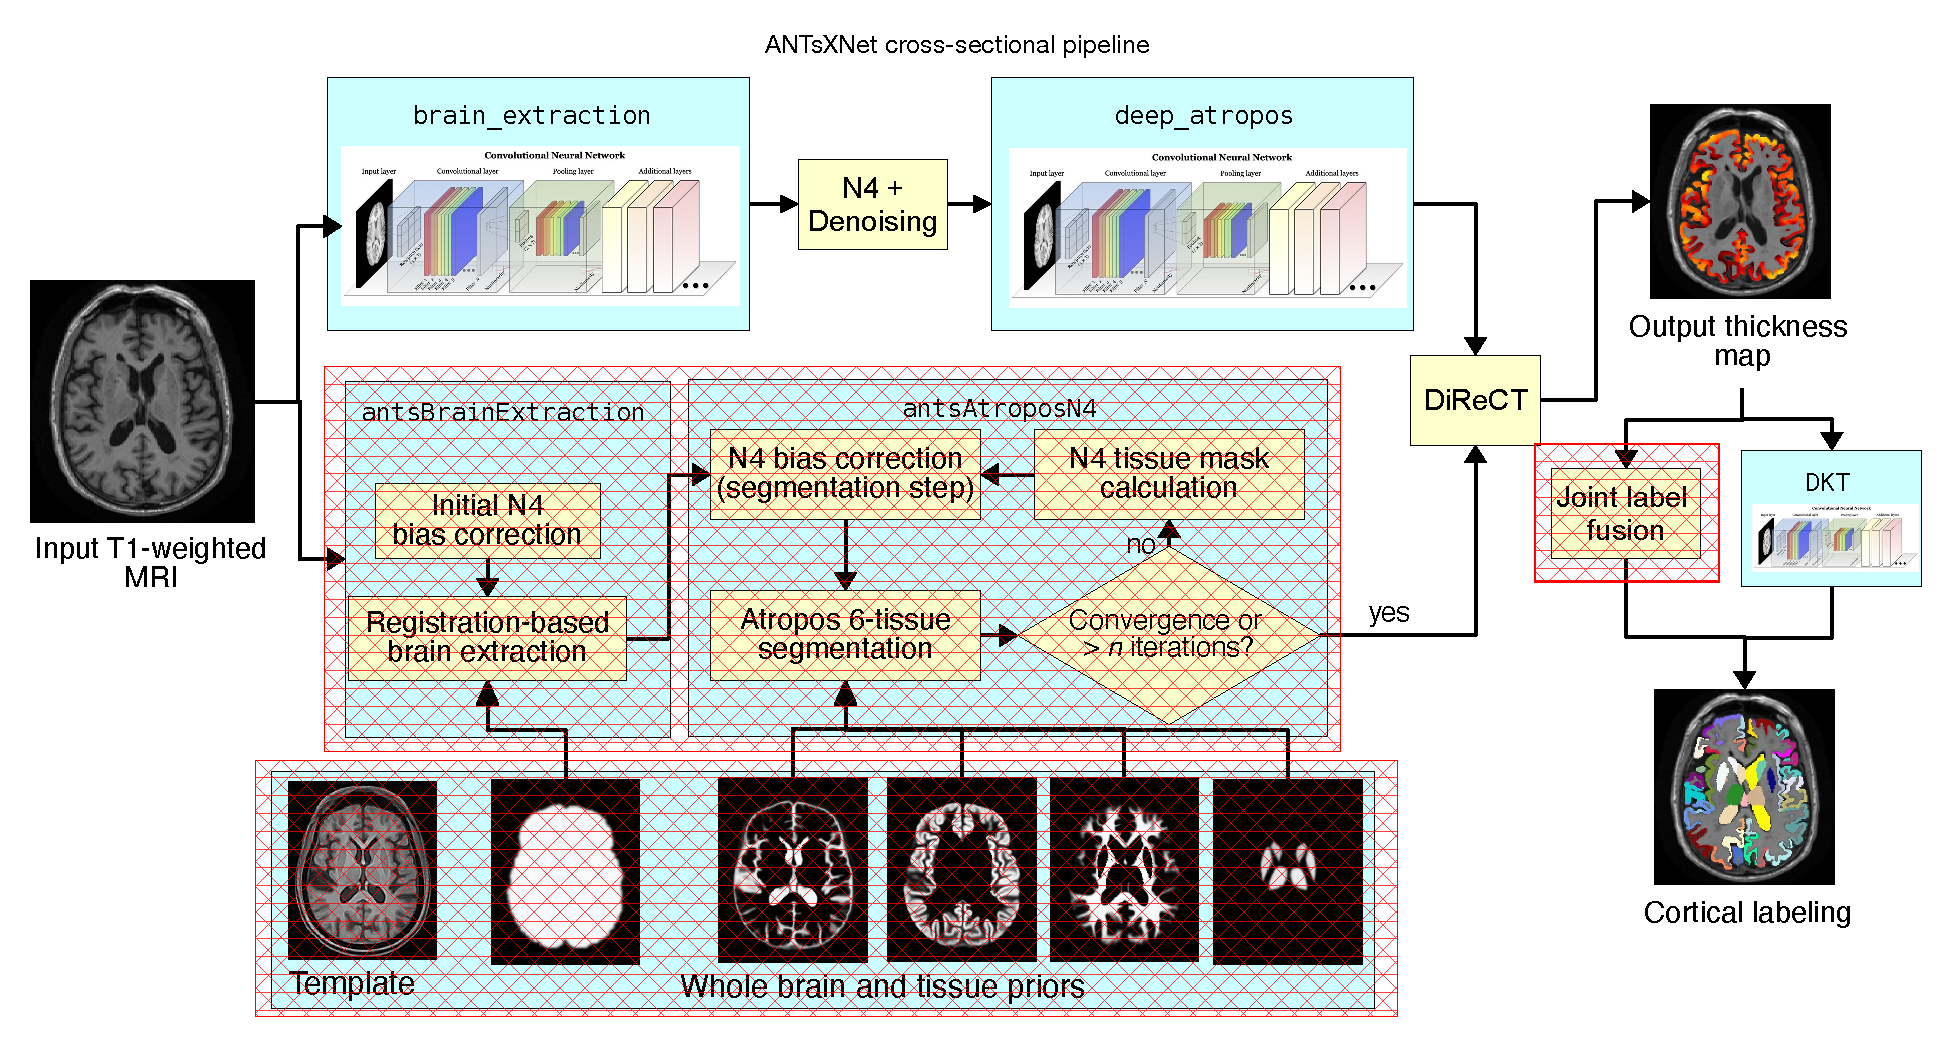
\includegraphics[width=\textwidth]{Figures/antsxnetPipeline.pdf}
  \caption{\textcolor{blue}{Illustration of the ANTsXNet cortical thickness pipeline and the
  relationship to its traditional ANTs analog.  The hash-designated sections
  denote pipeline steps which have been obviated by the deep learning approach.
  These include template-based brain extraction, template-based $n$-tissue
  segmentation, and joint label fusion for cortical labeling.}}
  \label{fig:pipeline}
\end{figure}

The most recent ANTsX
\textcolor{blue}{innovation involves the development of
deep learning analogs} of our popular ANTs cortical thickness
\textcolor{blue}{cross-sectional}\textsuperscript{16}
\textcolor{blue}{and
longitudinal}\textsuperscript{30} pipeline\textcolor{blue}{s} within the
ANTsXNet framework. \textcolor{blue}{Figure} \ref{fig:pipeline},
\textcolor{blue}{adapted from our previous work}\textsuperscript{16},
\textcolor{blue}{illustrates some of the major changes associated with the
single-subject pipeline.  The resulting improvement in efficiency
derives primarily from eliminating deformable image registration from the
pipeline---a step which has historically been used to propagate prior,
population-based information (e.g., tissue maps) to individual subjects for such
tasks as brain extraction}\textsuperscript{31}
\textcolor{blue}{and tissue
segmentation}\textsuperscript{10}
\textcolor{blue}{which is now configured within
the neural networks.}

\textcolor{blue}{These} structural MRI processing
pipeline\textcolor{blue}{s
are} currently available as open-source within the ANTsXNet libraries.
\textcolor{blue}{Evaluations using both cross-sectional and longitudinal data
are described in subsequent sections and couched} within the context of
our previous publications\textsuperscript{16,30}. Related work has been
recently reported by external groups\textsuperscript{32,33} and provide
a context for comparison to motivate the utility of the ANTsX ecosystem.

\hypertarget{results}{%
\section*{Results}\label{results}}
\addcontentsline{toc}{section}{Results}

\hypertarget{the-original-ants-cortical-thickness-pipeline}{%
\subsection*{The original ANTs cortical thickness
pipeline}\label{the-original-ants-cortical-thickness-pipeline}}
\addcontentsline{toc}{subsection}{The original ANTs cortical thickness
pipeline}

The original ANTs cortical thickness pipeline\textsuperscript{16}
consists of the following steps:

\begin{itemize}
\tightlist
\item
  preprocessing: denoising\textsuperscript{12} and bias
  correction\textsuperscript{34};
\item
  brain extraction\textsuperscript{31};
\item
  brain segmentation with spatial tissue priors\textsuperscript{10}
  comprising the

  \begin{itemize}
  \tightlist
  \item
    cerebrospinal fluid (CSF),
  \item
    gray matter (GM),
  \item
    white matter (WM),
  \item
    deep gray matter,
  \item
    cerebellum, and
  \item
    brain stem; and
  \end{itemize}
\item
  cortical thickness estimation\textsuperscript{15}.
\end{itemize}

Our recent longitudinal variant\textsuperscript{30} incorporates an
additional step involving the construction of a single subject template
(SST)\textsuperscript{9} coupled with the generation of tissue spatial
priors of the SST for use with the processing of the individual time
points as described above.

Although the resulting thickness maps are conducive to
voxel-based\textsuperscript{35} and related
analyses\textsuperscript{36}, here we employ the well-known
Desikan-Killiany-Tourville (DKT)\textsuperscript{37} labeling protocol
(31 labels per hemisphere) to parcellate the cortex for averaging
thickness values regionally (cf Table \ref{table:dkt_labels}). This
allows us to 1) be consistent in our evaluation strategy for comparison
with our previous work\textsuperscript{16,30} and 2) leverage an
additional deep learning-based substitution within the proposed
pipeline.

%\documentclass{standalone}
%\usepackage{booktabs}
%\begin{document}
%\begin{tabular*}{1\textwidth}{@{\extracolsep{\fill}} l l}
%  \toprule
%  \midrule
%  1) caudal anterior cingulate ({\tt cACC})  & 17) pars orbitalis ({\tt pORB}) \\
%  2) caudal middle frontal ({\tt cMFG})      & 18) pars triangularis ({\tt pTRI}) \\
%  3) cuneus ({\tt CUN})                      & 19) pericalcarine ({\tt periCAL}) \\
%  4) entorhinal ({\tt ENT})                  & 20) postcentral ({\tt postC}) \\
%  5) fusiform ({\tt FUS})                    & 21) posterior cingulate ({\tt PCC}) \\
%  6) inferior parietal ({\tt IPL})           & 22) precentral ({\tt preC}) \\
%  7) inferior temporal ({\tt ITG})           & 23) precuneus ({\tt PCUN}) \\
%  8) isthmus cingulate ({\tt iCC})           & 24) rosterior anterior cingulate ({\tt rACC}) \\
%  9) lateral occipital ({\tt LOG})           & 25) rostral middle frontal ({\tt rMFG}) \\
%  10) lateral orbitofrontal ({\tt LOF})      & 26) superior frontal ({\tt SFG}) \\
%  11) lingual ({\tt LING})                   & 27) superior parietal ({\tt SPL}) \\
%  12) medial orbitofrontal ({\tt MOF})       & 28) superior temporal ({\tt STG}) \\
%  13) middle temporal ({\tt MTG})            & 29) supramarginal ({\tt SMAR}) \\
%  14) parahippocampal ({\tt PARH})           & 30) transverse temporal ({\tt TT}) \\
%  15) paracentral ({\tt paraC})              & 31) insula ({\tt INS}) \\
%  16) pars opercularis  ({\tt pOPER})        & {}\\
%  \bottomrule
%\end{tabular*}
%\end{document}


\begin{table}[!htb]
\centering
\begin{tabular*}{0.95\textwidth}{@{\extracolsep{\fill}} l l}
 \toprule
 \midrule
 1) caudal anterior cingulate ({\tt cACC})  & 17) pars orbitalis ({\tt pORB}) \\
 2) caudal middle frontal ({\tt cMFG})      & 18) pars triangularis ({\tt pTRI}) \\
 3) cuneus ({\tt CUN})                      & 19) pericalcarine ({\tt periCAL}) \\
 4) entorhinal ({\tt ENT})                  & 20) postcentral ({\tt postC}) \\
 5) fusiform ({\tt FUS})                    & 21) posterior cingulate ({\tt PCC}) \\
 6) inferior parietal ({\tt IPL})           & 22) precentral ({\tt preC}) \\
 7) inferior temporal ({\tt ITG})           & 23) precuneus ({\tt PCUN}) \\
 8) isthmus cingulate ({\tt iCC})           & 24) rosterior anterior cingulate ({\tt rACC}) \\
 9) lateral occipital ({\tt LOG})           & 25) rostral middle frontal ({\tt rMFG}) \\
 10) lateral orbitofrontal ({\tt LOF})      & 26) superior frontal ({\tt SFG}) \\
 11) lingual ({\tt LING})                   & 27) superior parietal ({\tt SPL}) \\
 12) medial orbitofrontal ({\tt MOF})       & 28) superior temporal ({\tt STG}) \\
 13) middle temporal ({\tt MTG})            & 29) supramarginal ({\tt SMAR}) \\
 14) parahippocampal ({\tt PARH})           & 30) transverse temporal ({\tt TT}) \\
 15) paracentral ({\tt paraC})              & 31) insula ({\tt INS}) \\
 16) pars opercularis  ({\tt pOPER})        & {}\\
 \bottomrule
\end{tabular*}
\caption{The 31 cortical labels (per hemisphere) of the Desikan-Killiany-Tourville atlas.
        The ROI abbreviations from the R {\tt brainGraph} package are given in
        parentheses and used
        in later figures.
 }
\label{table:dkt_labels}
\end{table}


\hypertarget{overview-of-cortical-thickness-via-antsxnet}{%
\subsection*{Overview of cortical thickness via
ANTsXNet}\label{overview-of-cortical-thickness-via-antsxnet}}
\addcontentsline{toc}{subsection}{Overview of cortical thickness via
ANTsXNet}

The entire analysis/evaluation framework, from preprocessing to
statistical analysis, is made possible through the ANTsX ecosystem and
simplified through the open-source R and Python platforms.
Preprocessing, image registration, and cortical thickness estimation are
all available through the ANTsPy and ANTsR libraries whereas the deep
learning steps are performed through networks constructed and trained
via ANTsRNet/ANTsPyNet with data augmentation strategies and other
utilities built from ANTsR/ANTsPy functionality.

The brain extraction, brain segmentation, and DKT parcellation deep
learning components were trained using data derived from our previous
work\textsuperscript{16}. Specifically, the IXI\textsuperscript{38},
MMRR\textsuperscript{39}, NKI\textsuperscript{40}, and
OASIS\textsuperscript{41} data sets, and the corresponding derived data,
comprising over 1200 subjects from age 4 to 94, were used for network
training. Brain extraction employs a traditional 3-D U-net
network\textsuperscript{25} with whole brain, template-based data
augmentation\textsuperscript{24} whereas brain segmentation and DKT
parcellation are processed via 3-D U-net networks with attention
gating\textsuperscript{42} on image octant-based batches. We emphasize
that a single model (\textcolor{blue}{as opposed to ensemble
approaches where multiple models are used to produce the final solution}\textsuperscript{28})
was created for each of these steps and was used for all the experiments
described below.

\hypertarget{cross-sectional-performance-evaluation}{%
\subsection*{Cross-sectional performance
evaluation}\label{cross-sectional-performance-evaluation}}
\addcontentsline{toc}{subsection}{Cross-sectional performance
evaluation}

\begin{figure}[htb]
  \centering
    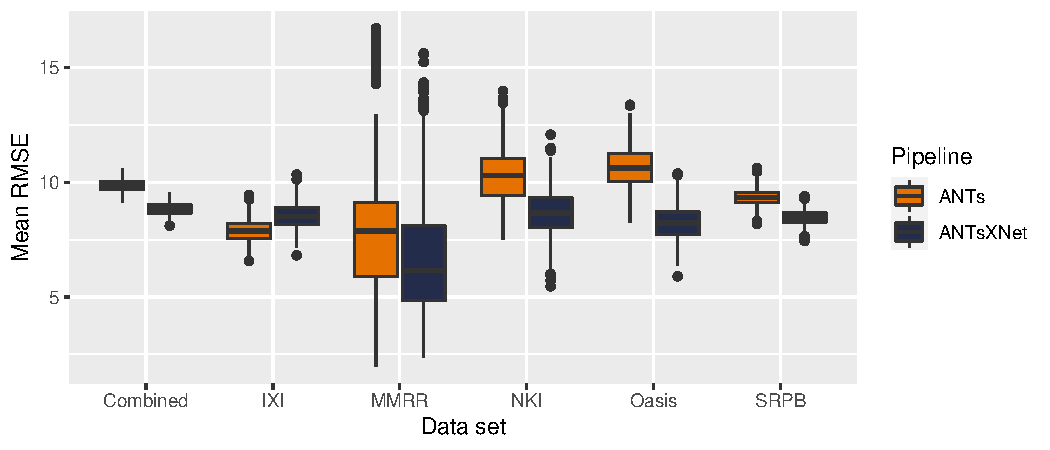
\includegraphics[width=\textwidth]{Figures/rmseThicknessPerSite.pdf}
  \caption{Distribution of mean RMSE values (500 permutations) for age
          prediction across the different data sets between
          the traditional ANTs and deep learning-based ANTsXNet pipelines. Total
          mean values are as follows: Combined---9.3 years (ANTs) and 8.2 years
          (ANTsXNet); IXI---7.9 years (ANTs) and 8.6 years (ANTsXNet);
          MMRR---7.9 years (ANTs) and 7.6 years (ANTsXNet); NKI---8.7 years
          (ANTs) and 7.9 years (ANTsXNet); OASIS---9.2 years (ANTs) and 8.0
          years (ANTsXNet); and SRPB---9.2 years (ANTs) and 8.1 years
          (ANTsXNet).}
  \label{fig:agePrediction}
\end{figure}

Due to the absence of ground-truth, we utilize the evaluation strategy
from our previous work\textsuperscript{16} where we used
cross-validation to build and compare age prediction models from data
derived from both the proposed ANTsXNet pipeline and the established
ANTs pipeline. Specifically, we use ``age'' as a well-known and
widely-available demographic correlate of cortical
thickness\textsuperscript{43} and quantify the predictive capabilities
of corresponding random forest classifiers\textsuperscript{44} of the
form: \begin{equation} AGE
\sim VOLUME + GENDER + \sum_{i=1}^{62} T(DKT_i) \end{equation} with
covariates \(GENDER\) and \(VOLUME\) (i.e., total intracranial volume).
\(T(DKT_i)\) is the average thickness value in the \(i^{th}\) DKT
region. Root mean square error (RMSE) between the actual and predicted
ages are the quantity used for comparative evaluation. As we have
explained previously\textsuperscript{16}, we find these evaluation
measures to be much more useful than other commonly applied criteria as
they are closer to assessing the actual utility of these thickness
measurements as biomarkers for disease\textsuperscript{45} or growth.
For example, in recent work\textsuperscript{32} the authors employ
correlation with FreeSurfer thickness values as the primary evaluation
for assessing relative performance with ANTs cortical
thickness\textsuperscript{16}. This evaluation, unfortunately, is
fundamentally flawed in that it is a prime example of a type of
circularity analysis\textsuperscript{46} whereby data selection is
driven by the same criteria used to evaluate performance. Specifically,
the underying DeepSCAN network used for the tissue segmentation step
employs training based on FreeSurfer results which directly influences
thickness values as thickness/segmentation are highly correlated and
vary characteristically between software packages. Relative performance
with ANTs thickness (which does not use FreeSurfer for training) is then
assessed by determining correlations with FreeSurfer thickness values.
Almost as problematic is their use of repeatability, which they
confusingly label as ``robustness,'' as an additional ranking criterion.
Repeatability evaluations should be contextualized within considerations
such as the bias-variance tradeoff and quantified using relevant
metrics, such as the intra-class correlation coefficient which takes
into account both inter- and intra-observer variability.

In addition to the training data listed above, to ensure
generalizability, we also compared performance using the SRPB data
set\textsuperscript{47} comprising over 1600 participants from 12 sites.
Note that we recognize that we are processing a portion of the
evaluation data through certain components of the proposed deep
learning-based pipeline that were used to train the same pipeline
components. Although this does not provide evidence for generalizability
(which is why we include the much larger SRPB data set), it is still
interesting to examine the results since, in this case, the deep
learning training can be considered a type of noise reduction on the
final results. It should be noted that training did not use age
prediction (or any other evaluation or related measure) as a criterion
to be optimized during network model training (i.e., circular
analysis\textsuperscript{46}).

The results are shown in Figure \ref{fig:agePrediction} where we used
cross-validation with 500 permutations per model per data set (including
a ``combined'' set) and an 80/20 training/testing split. The ANTsXNet
deep learning pipeline outperformed the classical
pipeline\textsuperscript{16} in terms of age prediction in all data sets
except for IXI. This also includes the cross-validation iteration where
all data sets were combined. Importance plots ranking the cortical
thickness regions and the other covariates of Equation (1) are shown in
Figure \ref{fig:rfimportance}. Rankings employ ``MeanDecreaseAccuracy''
which quantifies the decrease in model accuracy based on the exclusion
of a specific random forest regressor. Additionally, repeatability
assessment on the MMRR data set yielded ICC values (``average random
rater'') of 0.99 for both pipelines.

\begin{figure}[htb]
  \centering
  \begin{subfigure}{0.4\textwidth}
    \centering
    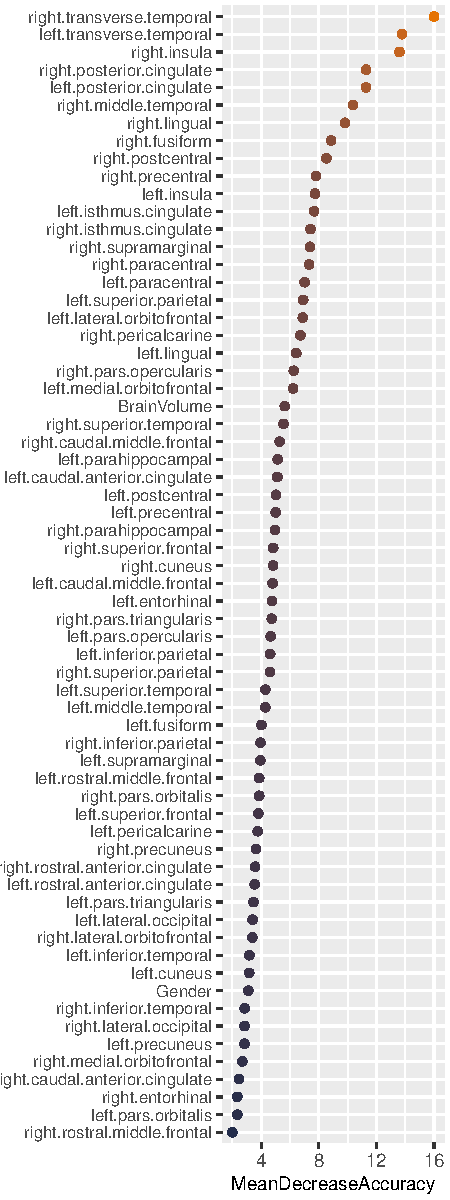
\includegraphics[width=0.75\linewidth]{Figures/rfImportance_SRPB1600_ANTs.pdf}
    \caption{ANTs}
  \end{subfigure}%
  \begin{subfigure}{0.4\textwidth}
    \centering
    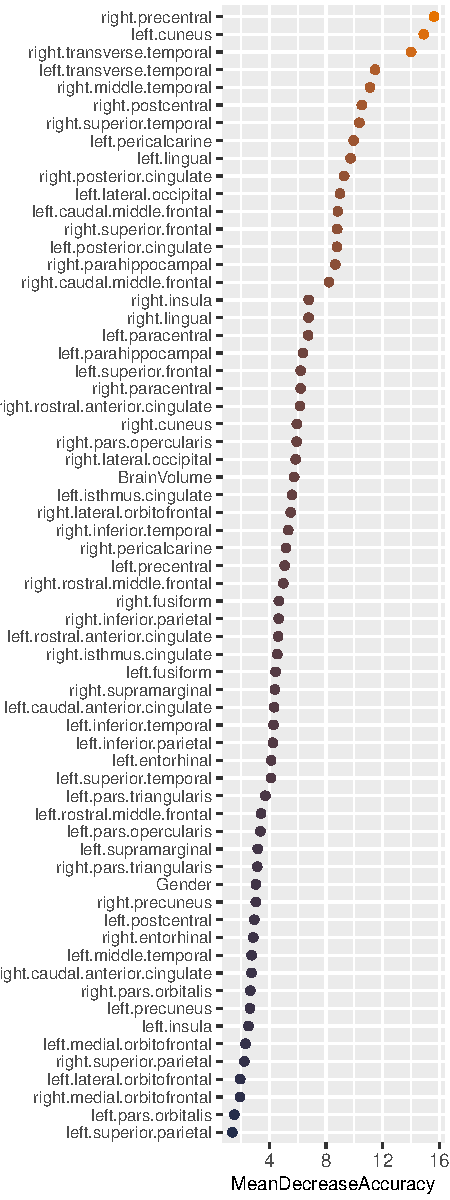
\includegraphics[width=0.75\linewidth]{Figures/rfImportance_SRPB1600_ANTsXNet.pdf}
    \caption{ANTsXNet}
  \end{subfigure}
\caption{Importance plots for the SRPB data set using ``MeanDecreaseAccuracy'' for the
random forest regressors (i.e., cortical thickness regions, gender, and brain volume
specified by Equation (1).}
\label{fig:rfimportance}
\end{figure}

\hypertarget{longitudinal-performance-evaluation}{%
\subsection*{Longitudinal performance
evaluation}\label{longitudinal-performance-evaluation}}
\addcontentsline{toc}{subsection}{Longitudinal performance evaluation}

\begin{figure}[!htb]
  \centering
  \begin{subfigure}{0.95\textwidth}
    \centering
    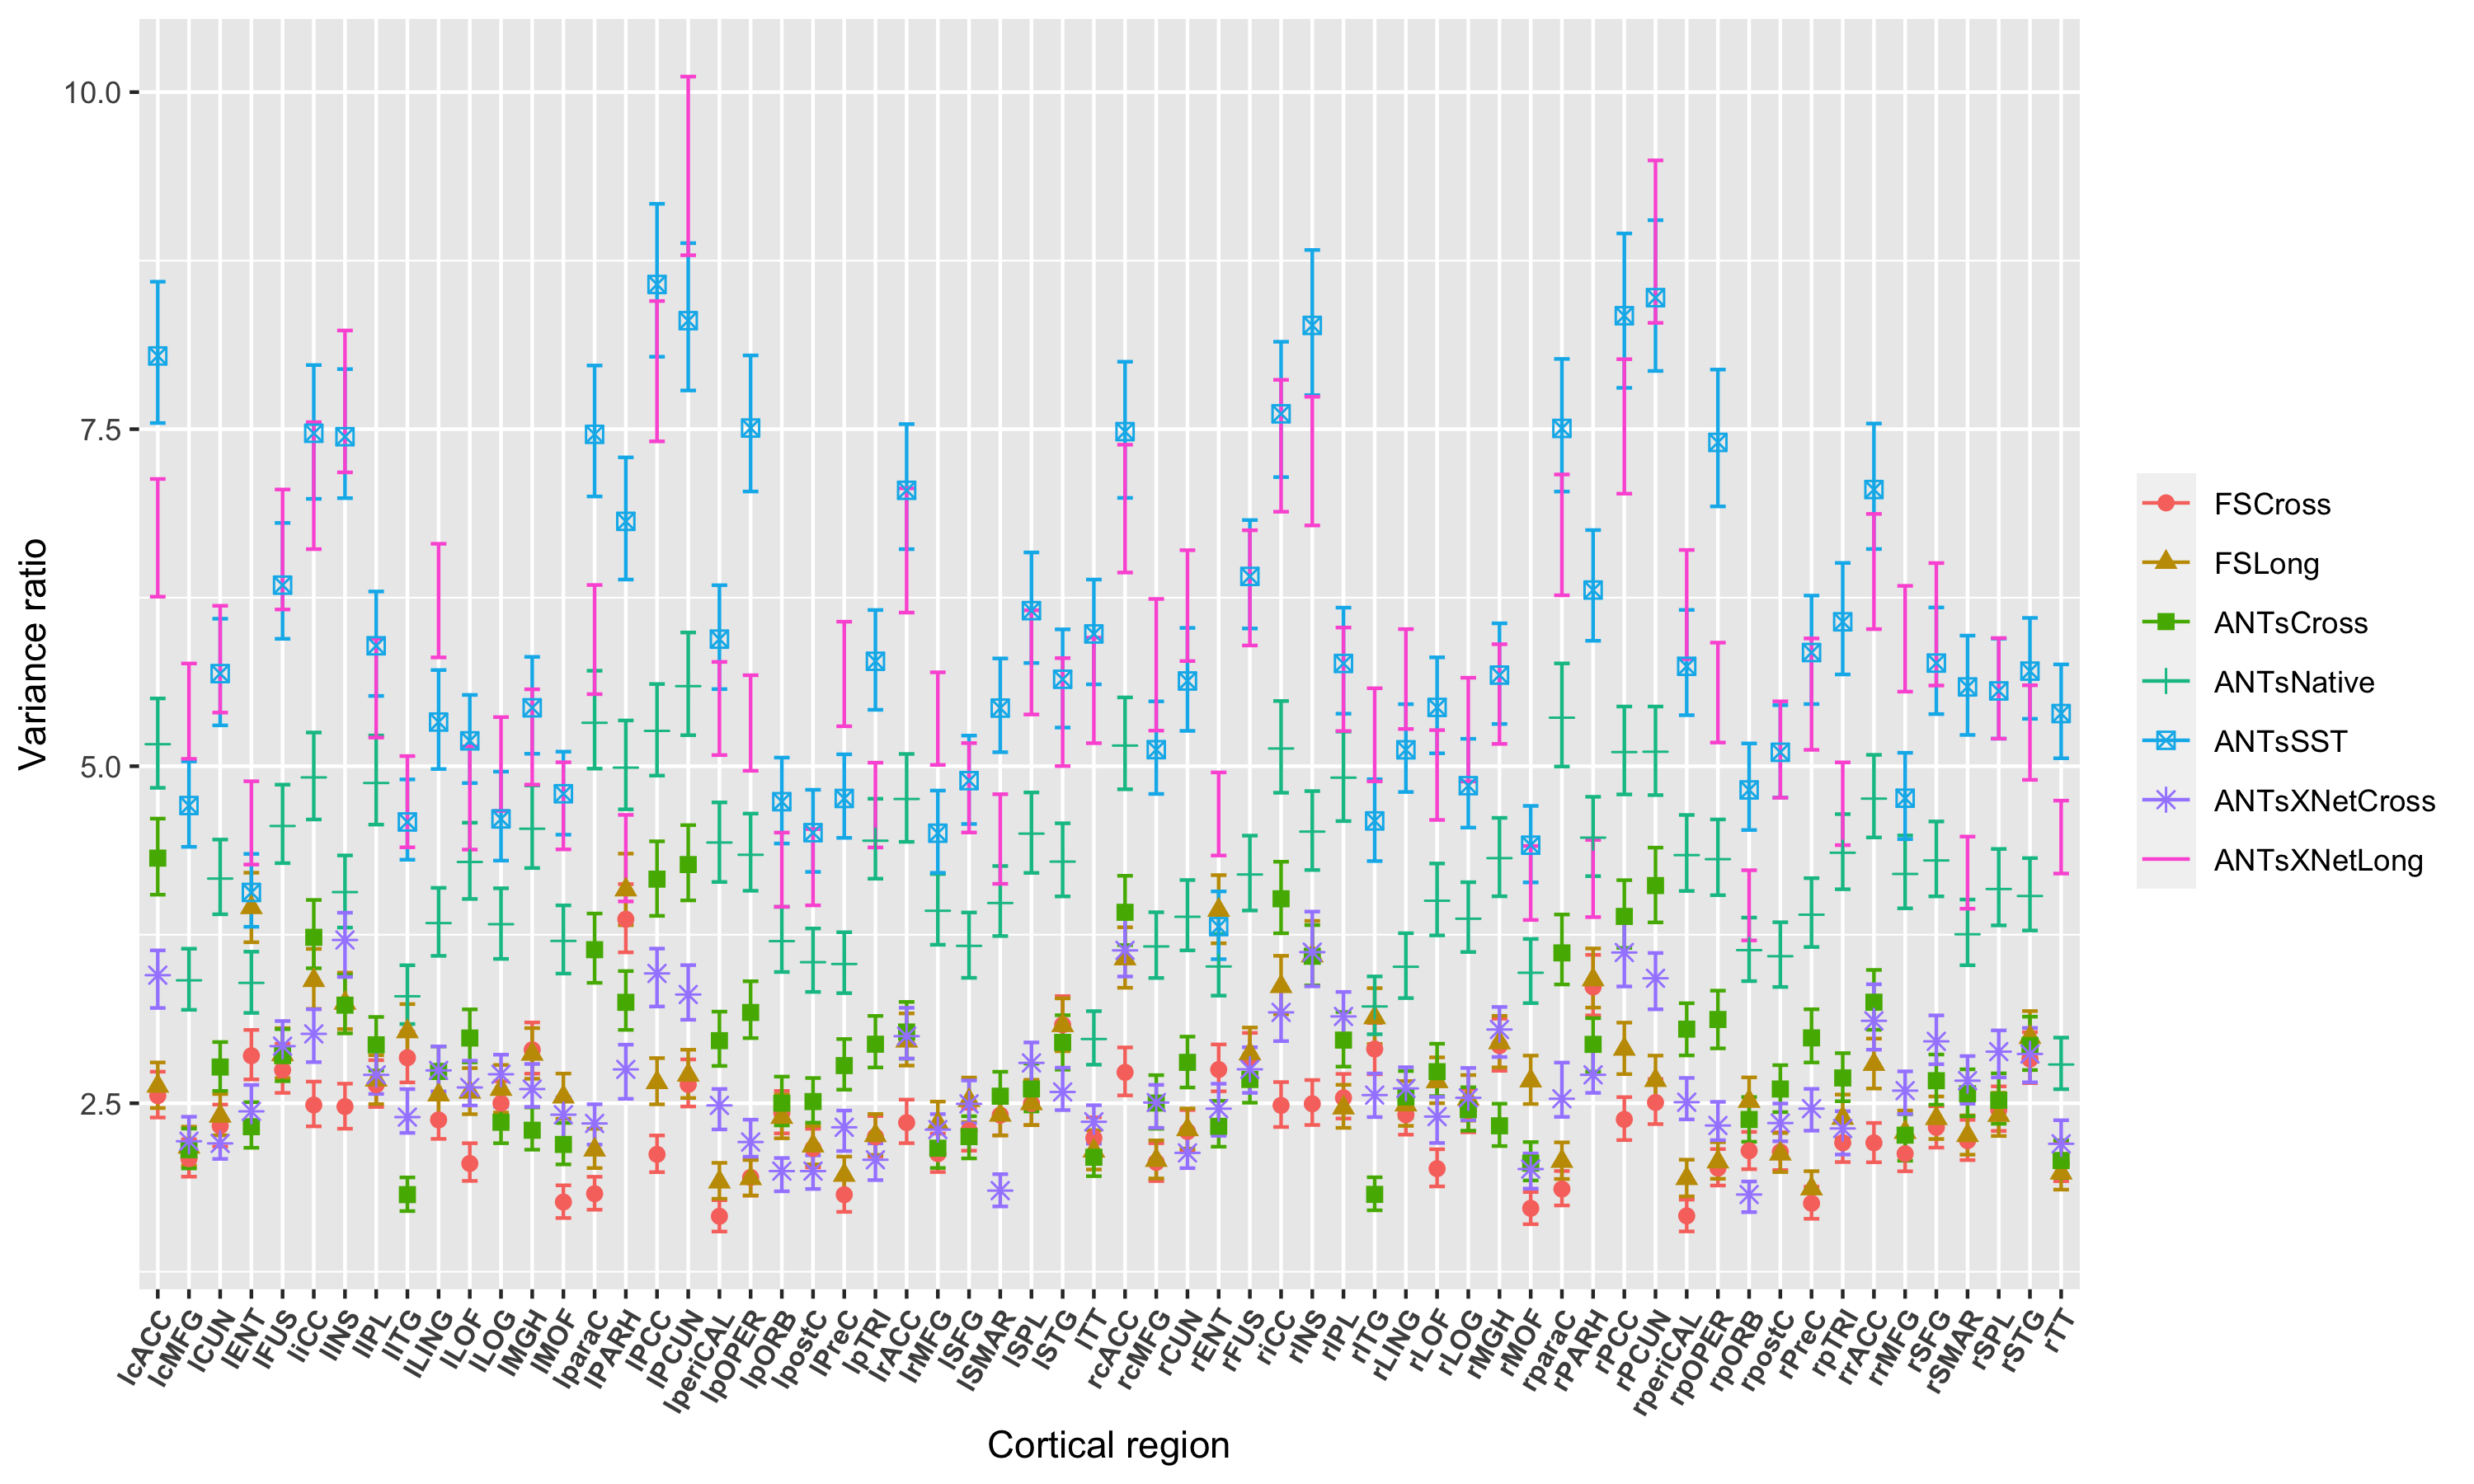
\includegraphics[width=1.0\linewidth]{Figures/variance.ratio_FINALX.png}
    \caption{}
  \end{subfigure}
  \begin{subfigure}{0.95\textwidth}
    \centering
    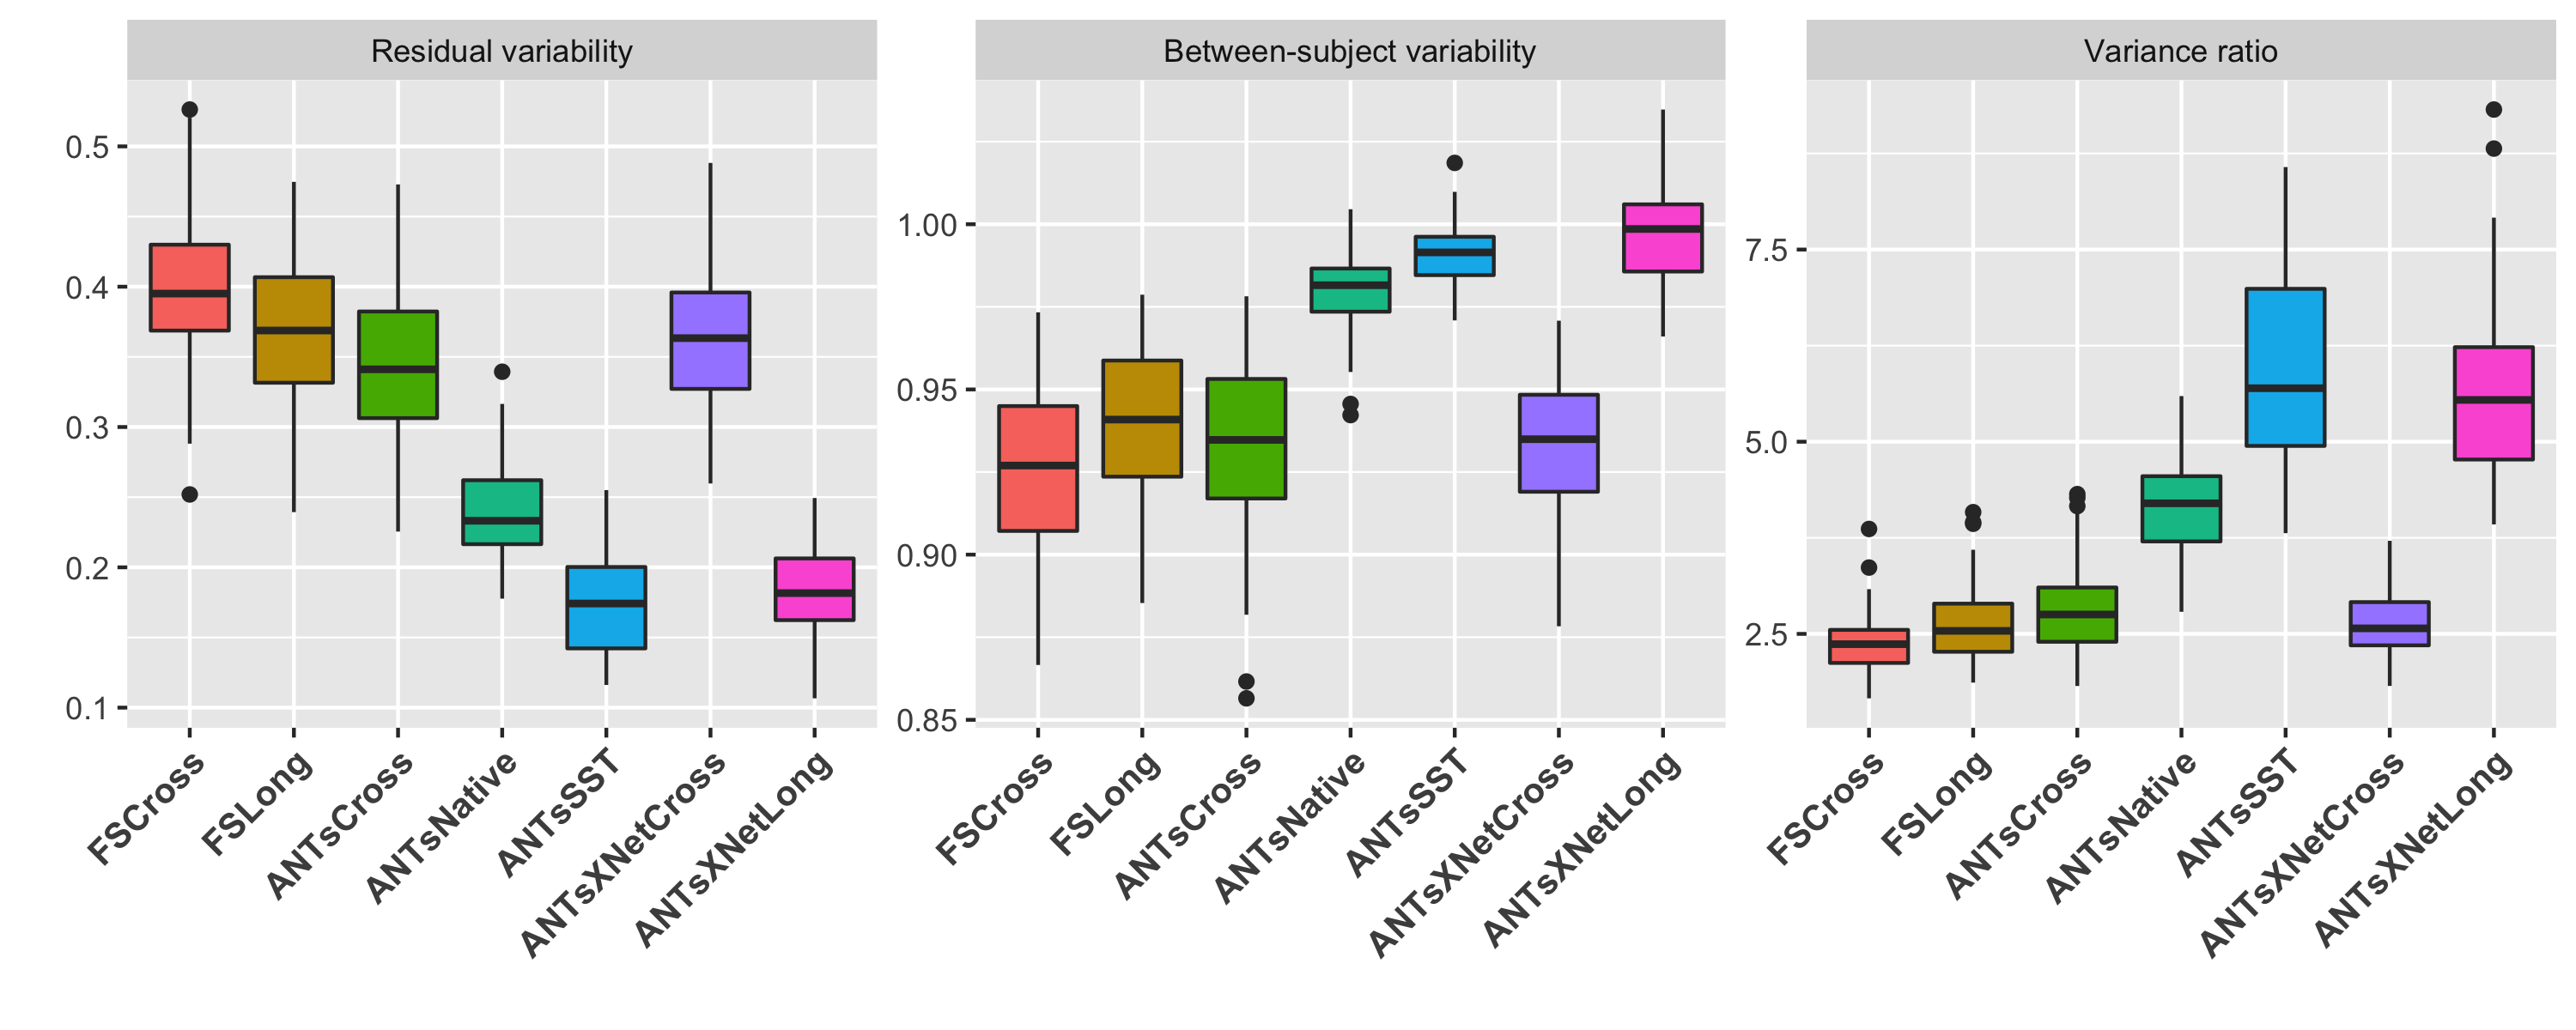
\includegraphics[width=1\linewidth]{Figures/allData_FINALX2.png}
    \caption{}
  \end{subfigure}
  \caption{Performance over longitudinal data as determined by the variance ratio.
    (a) Region-specific 95\% confidence intervals of the variance ratio showing the
    superior performance of the longitudinally tailored ANTsX-based pipelines, including
    ANTsSST and ANTsXNetLong. (b) Residual variability, between subject, and variance ratio
    values per pipeline over all DKT regions. }
\label{fig:longeval1}
\end{figure}

\begin{figure}[!htb]
  \centering
    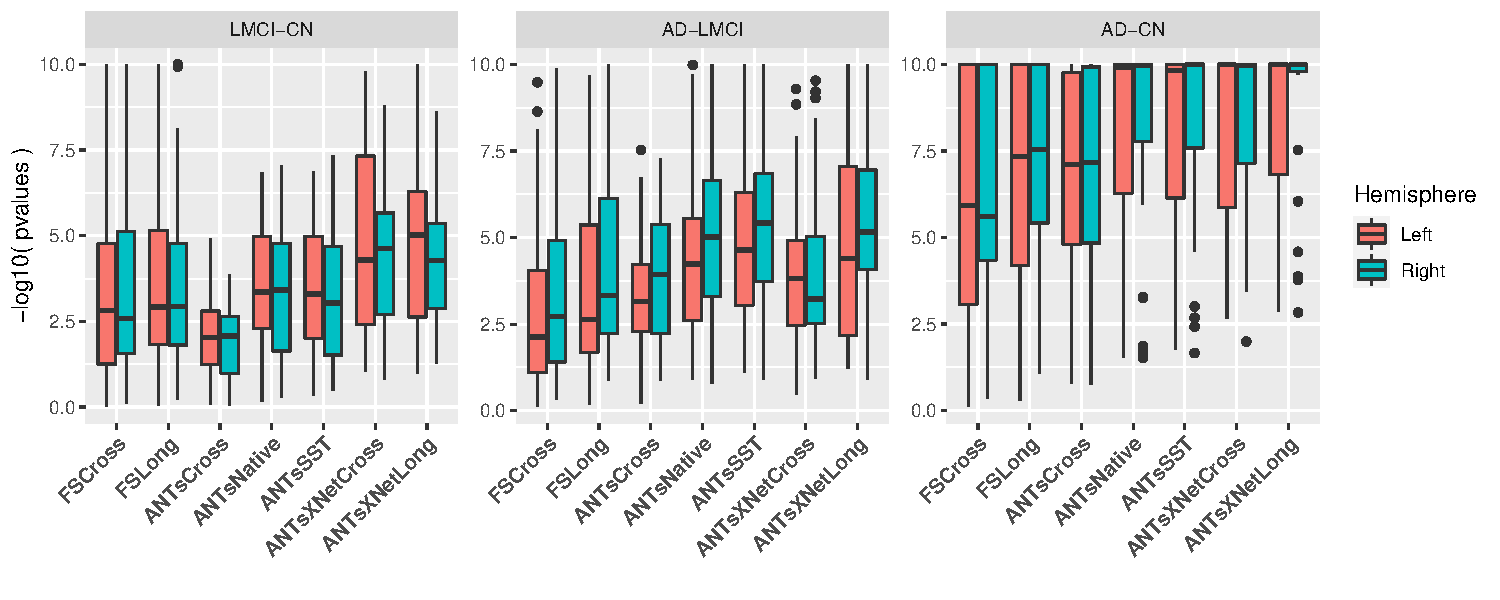
\includegraphics[width=1.0\linewidth]{Figures/logPvalues2.pdf}
  \caption{Measures for the supervised evaluation
  strategy where log p-values for diagnostic
  differentiation of LMCI-CN, AD-LMCI, and AD-CN subjects are plotted for all pipelines
  over all DKT regions. }
  \label{fig:longeval2}
\end{figure}

Given the excellent performance and superior computational efficiency of
the proposed ANTsXNet pipeline for cross-sectional data, we evaluated
its performance on longitudinal data using the longitudinally-specific
evaluation strategy and data we employed with the introduction of the
longitudinal version of the ANTs cortical thickness
pipeline\textsuperscript{30}. \textcolor{blue}{
We also evaluated an ANTsXNet-based pipeline tailored specifically for longitudinal
data.  In this variant, an SST is generated and processed using the previously
described ANTsXNet cross-sectional pipeline which yields tissue spatial priors.
These spatial priors are used in our traditional brain segmentation approach}\textsuperscript{10}\textcolor{blue}{.  The computational efficiency of this variant is also
significantly improved due to the elimination of the costly SST prior generation
which uses multiple registrations combined with joint label fusion}\textsuperscript{14}.

The ADNI-1 data used for our longitudinal performance
evaluation\textsuperscript{30} consisted of over 600 subjects (197
cognitive normals, 324 LMCI subjects, and 142 AD subjects) with one or
more follow-up image acquisition sessions every 6 months (up to 36
months) for a total of over 2500 images. In addition to the ANTsXNet
pipelines \textcolor{blue}{(``ANTsXNetCross'' and
``ANTsXNetLong'')} for the current evaluation, our previous work
included the FreeSurfer\textsuperscript{23} cross-sectional
(``FSCross'') and longitudinal (``FSLong'') streams, the ANTs
cross-sectional pipeline (``ANTsCross'') in addition to two longitudinal
ANTs-based variants (``ANTsNative'' and ``ANTsSST''). Two evaluation
measurements, one unsupervised and one supervised, were used to assess
comparative performance between all seven pipelines. We add the results
of the ANTsXNet pipeline
\textcolor{blue}{cross-sectional and longitudinal} evaluations in
relation to these other pipelines to provide a comprehensive overview of
relative performance.

First, \textcolor{blue}{linear mixed-effects} (LME)\textsuperscript{48}
modeling was used to quantify between-subject and residual
variabilities, the ratio of which provides an estimate of the
effectiveness of a given biomarker for distinguishing between
subpopulations. In order to assess this criteria while accounting for
changes that may occur through the passage of time, we used the
following Bayesian LME model: \begin{gather}
  Y^k_{ij} \sim N(\alpha^k_i + \beta^k_i t_{ij}, \sigma_k^2) \\ \nonumber
  \alpha^k_i \sim N(\alpha^k_0, \tau^2_k) \,\,\,\, \beta^k_i \sim N(\beta^k_0, \rho^2_k) \\ \nonumber
  \alpha^k_0, \beta^k_0 \sim N(0,10) \,\,\,\,  \sigma_k, \tau_k, \rho_k \sim \mbox{Cauchy}^+ (0, 5)
\end{gather} where \(Y^k_{ij}\) denotes the \(i^{th}\) individual's
cortical thickness measurement corresponding to the \(k^{th}\) region of
interest at the time point indexed by \(j\) and specification of
variance priors to half-Cauchy distributions reflects commonly accepted
best practice in the context of hierarchical models\textsuperscript{49}.
The ratio of interest, \(r^k\), per region of the between-subject
variability, \(\tau_k\), and residual variability, \(\sigma_k\) is
\begin{align}
  r^k = \frac{\tau_k}{\sigma_k}, k = 1,\ldots,62
\end{align} where the posterior distribution of \(r_k\) was summarized
via the posterior median.

Second, the supervised evaluation employed Tukey post-hoc analyses with
false discovery rate (FDR) adjustment to test the significance of the
LMCI-CN, AD-LMCI, and AD-CN diagnostic contrasts. This is provided by
the following LME model \begin{align}
  \Delta Y \sim & Y_{bl} + AGE_{bl} + ICV_{bl} + APOE_{bl} + GENDER + DIAGNOSIS_{bl} \\ \nonumber
                & + VISIT:DIAGNOSIS_{bl} + (1 | ID) + (1 | SITE).
\end{align} Here, \(\Delta Y\) is the change in thickness of the
\(k^{th}\) DKT region from baseline (bl) thickness \(Y_{bl}\) with
random intercepts for both the individual subject (\(ID\)) and the
acquisition site. The subject-specific covariates \(AGE\), \(APOE\)
status, \(GENDER\), \(DIAGNOSIS\), \(ICV\), and \(VISIT\) were taken
directly from the ADNIMERGE package.

\textcolor{blue}{Results for all pipelines with respect to the longitudinal
evaluation criteria are shown in Figures \ref{fig:longeval1} and
\ref{fig:longeval2}.  Figure \ref{fig:longeval1}(a) provides the 95\% confidence
intervals of the variance ratio for all 64 regions of the DKT cortical labeling
where ANTsSST consistently performs best with ANTsXNetLong also performing
well.  These quantities are summarized in Figure \ref{fig:longeval1}(b).  The
second evaluation criteria compares diagnostic differentiation via LMEs.  Log
p-values are provided in Figure \ref{fig:longeval2} which demonstrate excellent
LMCI-CN and AD-CN differentiation for both deep learning pipelines.}

\hypertarget{discussion}{%
\section*{Discussion}\label{discussion}}
\addcontentsline{toc}{section}{Discussion}

The ANTsX software ecosystem provides a comprehensive framework for
quantitative biological and medical imaging. Although ANTs, the original
core of ANTsX, is still at the forefront of image registration
technology, it has moved signicantly beyond its image registration
origins. This expansion is not confined to technical contributions (of
which there are many) but also consists of facilitating access to a wide
range of users who can use ANTsX tools (whether through bash, Python, or
R scripting) to construct tailored pipelines for their own studies or to
take advantage of our pre-fabricated pipelines. And given the
open-source nature of the ANTsX software, usage is not limited, for
example, to academic institutions---a common constraint characteristic
of other packages.

One of our most widely used pipelines is the estimation of cortical
thickness from neuroimaging. This is understandable given the widespread
usage of regional cortical thickness as a biomarker for developmental or
pathological trajectories of the brain. In this work, we used this
well-vetted ANTs tool to provide training data for producing alternative
variants which leverage deep learning for improved computational
efficiency and also provides superior performance with respect to
previously proposed evaluation measures for both
cross-sectional\textsuperscript{16} and longitudinal
scenarios\textsuperscript{30}. In addition to providing the tools which
generated the original training data for the proposed ANTsXNet pipeline,
the ANTsX ecosystem provides a full-featured platform for the additional
steps such as preprocessing (ANTsR/ANTsPy); data augmentation
(ANTsR/ANTsPy); network construction and training (ANTsRNet/ANTsPyNet);
and visualization and statistical analysis of the results
(ANTsR/ANTsPy).

\textcolor{blue}{It is the comprehensiveness of ANTsX that provides significant
advantages over much of the deep learning work that is currently taking place in
medical imaging. In other words, various steps in the deep learning training
processing (e.g., data augmentation, preprocessing) can all be performed within
the same ecosystem where such important details as header information for image
geometry are treated the same.} In contrast, related
work\textsuperscript{32} described and evaluated a similar thickness
measurement pipeline. However, due to the lack of a complete processing
and analysis framework, training data was generated using the FreeSurfer
stream, deep learning-based brain segmentation employed
DeepSCAN\textsuperscript{50} (in-house software), and cortical thickness
estimation\textsuperscript{15} was generated using the ANTs toolkit.
\textcolor{blue}{For the reader interested in reproducing the authors' results,
they are primarily prevented from doing so due, as far as we can tell, to the
lack of the public availability of the DeepSCAN software. However, in addition,
the interested reader must also ensure the consistency of the input/output
interface between packages (a task for which the Nipype development team is
quite familiar.)}

In terms of future work, the recent surge and utility of deep learning
in medical image analysis has significantly guided the areas of active
ANTsX development. As demonstrated in this work with our widely used
cortical thickness pipelines, there are many potential benefits of deep
learning analogs to existing ANTs tools as well as the development of
new ones. Performance is \textcolor{blue}{mostly} comparable-to-superior
relative to existing pipelines depending on the evaluation metric.
\textcolor{blue}{Specifically, the ANTsXNet
cross-sectional pipeline does well for the age prediction performance framework
and in terms of the ICC.  Additionally, this pipeline performs relatively well
for longitudinal ADNI data for disease differentiation but not so much in terms
of the generic variance ratio criterion.  However, for such longitudinal-specific
studies, the ANTsXNet longitudinal variant performs well for both performance
measures.} We see possible additional longitudinal extensions
incorporating subject ID and months as additional network inputs.

\hypertarget{methods}{%
\section*{Methods}\label{methods}}
\addcontentsline{toc}{section}{Methods}

Software, average DKT regional thickness values for all data sets, and
the scripts to perform both the analysis and obtain thickness values for
a single subject \textcolor{blue}{(cross-sectionally or longitudinally)}
are provided as open-source. Specifically, all the ANTsX libraries are
hosted on GitHub (\url{https://github.com/ANTsX}). The cross-sectional
data and analysis code are available as .csv files and R scripts at the
GitHub repository dedicated to this paper
(\url{https://github.com/ntustison/PaperANTsX}) whereas the longitudinal
data and evaluation scripts are organized with the repository associated
with our previous work\textsuperscript{30}
(\url{https://github.com/ntustison/CrossLong}).

\hypertarget{implementation}{%
\subsection*{Implementation}\label{implementation}}
\addcontentsline{toc}{subsection}{Implementation}

\vspace{10mm}

\setstretch{1.0}

\lstset{frame = htb,
        framerule = 0.25pt,
        float,
        fontadjust,
        backgroundcolor={\color{listlightgray}},
        basicstyle = {\ttfamily\scriptsize},
        keywordstyle = {\ttfamily\color{listkeyword}\textbf},
        identifierstyle = {\ttfamily},
        commentstyle = {\ttfamily\color{listcomment}\textit},
        stringstyle = {\ttfamily},
        showstringspaces = false,
        showtabs = false,
        numbers = none,
        numbersep = 6pt,
        numberstyle={\ttfamily\color{listnumbers}},
        tabsize = 2,
        language=python,
        floatplacement=!h,
        caption={\small ANTsPy/ANTsPyNet command calls
        for a single IXI subject in the evaluation study for
        the cross-sectional pipeline.
        },
        captionpos=b,
        label=listing:antspyCorticalThickness
        }
\begin{lstlisting}
import ants
import antspynet

# ANTsPy/ANTsPyNet processing for subject IXI002-Guys-0828-T1
t1_file = "IXI002-Guys-0828-T1.nii.gz"
t1 = ants.image_read(t1_file)

# Atropos six-tissue segmentation
atropos = antspynet.deep_atropos(t1, do_preprocessing=True, verbose=True)

# Kelly Kapowski cortical thickness (combine Atropos WM and deep GM)
kk_segmentation = atropos['segmentation_image']
kk_segmentation[kk_segmentation == 4] = 3
kk_gray_matter = atropos['probability_images'][2]
kk_white_matter = atropos['probability_images'][3] + atropos['probability_images'][4]
kk = ants.kelly_kapowski(s=kk_segmentation, g=kk_gray_matter, w=kk_white_matter,
                         its=45, r=0.025, m=1.5, x=0, verbose=1)

# Desikan-Killiany-Tourville labeling
dkt = antspynet.desikan_killiany_tourville_labeling(t1, do_preprocessing=True, verbose=True)

# DKT label propagation throughout the cortex
dkt_cortical_mask = ants.threshold_image(dkt, 1000, 3000, 1, 0)
dkt = dkt_cortical_mask * dkt
kk_mask = ants.threshold_image(kk, 0, 0, 0, 1)
dkt_propagated = ants.iMath(kk_mask, "PropagateLabelsThroughMask", kk_mask * dkt)

# Get average regional thickness values
kk_regional_stats = ants.label_stats(kk, dkt_propagated)
\end{lstlisting}

\setstretch{1.5}

In Listing 1, we show the ANTsPy/ANTsPyNet code snippet for
cross-sectional processing a single subject which starts with reading
the T1-weighted MRI input image, through the generation of the
Atropos-style six-tissue segmentation and probability images,
application of \texttt{ants.kelly\_kapowski} (i.e., DiReCT), DKT
cortical parcellation, subsequent label propagation through the cortex,
and, finally, regional cortical thickness tabulation.
\textcolor{blue}{The
cross-sectional and longitudinal pipelines are encapsulated in the ANTsPyNet
functions} \texttt{antspynet.cortical\_thickness} and
\texttt{antspynet.longitudinal\_cortical\_thickness},
\textcolor{blue}{respectively.} Note that there are precise,
line-by-line R-based analogs available through ANTsR/ANTsRNet.

Both the \texttt{ants.deep\_atropos} and
\texttt{antspynet.desikan\_killiany\_tourville\_labeling} functions
perform brain extraction using the \texttt{antspynet.brain\_extraction}
function. Internally, \texttt{antspynet.brain\_extraction} contains the
requisite code to build the network and assign the appropriate
hyperparameters. The model weights are automatically downloaded from the
online hosting site \url{https://figshare.com} (see the function
\texttt{get\_pretrained\_network} in ANTsPyNet or
\texttt{getPretrainedNetwork} in ANTsRNet for links to all models and
weights) and loaded to the constructed network.
\texttt{antspynet.brain\_extraction} performs a quick translation
transformation to a specific template (also downloaded automatically)
using the centers of intensity mass, a common alignment initialization
strategy. This is to ensure proper gross orientation. Following brain
extraction, preprocessing for the other two deep learning components
includes \texttt{ants.denoise\_image} and
\texttt{ants.n4\_bias\_correction} and an affine-based reorientation to
a version of the MNI template\textsuperscript{51}.

We recognize the presence of some redundancy due to the repeated
application of certain preprocessing steps. Thus, each function has a
\texttt{do\_preprocessing} option to eliminate this redundancy for
knowledgeable users but, for simplicity in presentation purposes, we do
not provide this modified pipeline here. Although it should be noted
that the time difference is minimal considering the longer time required
by \texttt{ants.kelly\_kapowski}. \texttt{ants.deep\_atropos} returns
the segmentation image as well as the posterior probability maps for
each tissue type listed previously.
\texttt{antspynet.desikan\_killiany\_tourville\_labeling} returns only
the segmentation label image which includes not only the 62 cortical
labels but the remaining labels as well. The label numbers and
corresponding structure names are given in the program description/help.
Because the DKT parcellation will, in general, not exactly coincide with
the non-zero voxels of the resulting cortical thickness maps, we perform
a label propagation step to ensure the entire cortex, and only the
non-zero thickness values in the cortex, are included in the tabulated
regional values.

\textcolor{blue}{As mentioned previously, the longitudinal version,}
\texttt{antspynet.longitudinal\_cortical\_thickness},
\textcolor{blue}{adds an SST
generation step which can either be provided as a program input or it can be
constructed from spatial normalization of all time points to a specified
template.} \texttt{ants.deep\_atropos}
\textcolor{blue}{is applied to the SST
yielding spatial tissues priors which are then used as input to}
\texttt{ants.atropos} \textcolor{blue}{for each time point. }
\texttt{ants.kelly\_kapowski}
\textcolor{blue}{is applied to the result to generate the desired cortical
thickness maps.}

\textcolor{blue}{Computational time on a CPU-only platform is approximately 1
hour primarily due to} \texttt{ants.kelly\_kapowski}
\textcolor{blue}{processing.
Other preprocessing steps, i.e., bias correction and denoising, are on the order of a
couple minutes. This total time should be compared with $4-5$ hours
using the traditional pipeline employing the} \texttt{quick}
\textcolor{blue}{registration option or $10-15$ hours with the more
comprehensive registration parameters employed).  As mentioned previously,
elimination of the registration-based propagation of prior probability images to
individual subjects is the principal source of reduced computational time. For
ROI-based analyses, this is in addition to the elimination of the optional
generation of a population-specific template. Additionally, the use of}
\texttt{antspynet.desikan\_killiany\_tourville\_labeling},
\textcolor{blue}{for cortical
labeling (which completes in less than five minutes) eliminates the need for
joint label fusion which requires multiple pairwise registrations for each
subject in addition to the fusion algorithm itself.}

\hypertarget{training-details}{%
\subsection*{Training details}\label{training-details}}
\addcontentsline{toc}{subsection}{Training details}

Training differed slightly between models and so we provide details for
each of these components below. For all training, we used ANTsRNet
scripts and custom batch generators. Although the network construction
and other functionality is available in both ANTsPyNet and ANTsRNet (as
is model weights compatibility), we have not written such custom batch
generators for the former (although this is on our to-do list). In terms
of hardware, all training was done on a DGX (GPUs: 4X Tesla V100, system
memory: 256 GB LRDIMM DDR4).

\textbf{T1-weighted brain extraction.} A whole-image 3-D U-net
model\textsuperscript{25} was used in conjunction with multiple training
sessions employing a Dice loss function followed by categorical cross
entropy. \textcolor{blue}{Training data
was derived from the same multi-site data described previously processed through
our registration-based approach}\textsuperscript{31}. A
center-of-mass-based transformation to a standard template was used to
standardize such parameters as orientation and voxel size. However, to
account for possible different header orientations of input data, a
template-based data augmentation scheme was used\textsuperscript{24}
whereby forward and inverse transforms are used to randomly warp batch
images between members of the training population (followed by
reorientation to the standard template). A digital random coin flipping
for possible histogram matching\textsuperscript{52} between source and
target images further increased data augmentation.
\textcolor{blue}{The output of the network
is a probabilistic mask of the brain.} Although not detailed here,
training for brain extraction in other modalities was performed
similarly.

\textbf{Deep Atropos.} Dealing with 3-D data presents unique barriers
for training that are often unique to medical imaging. Various
strategies are employed such as minimizing the number of layers and/or
the number of filters at the base layer of the U-net architecture (as we
do for brian extraction). However, we found this to be too limiting for
capturing certain brain structures such as the cortex. 2-D and 2.5-D
approaches are often used with varying levels of success but we also
found better performance using full 3-D information. This led us to try
randomly selected 3-D patches of various sizes. However, for both the
six-tissue segmentations and DKT parcellations, we found that an
octant-based patch strategy yielded the desired results. Specifically,
after a brain extracted affine normalization to the MNI template, the
normalized image is cropped to a size of {[}160, 190, 160{]}.
Overlapping octant patches of size {[}112, 112, 112{]} were extracted
from each image and trained using a batch size of 12 such octant patches
with weighted categorical cross entropy as the loss function. As we
point out in our earlier work\textsuperscript{16}, obtaining proper
brain segmentation is perhaps the most critical step to estimating
thickness values that have the greatest utility as a potential
biomarker. In fact, the first and last authors (NT and BA, respectively)
spent much time during the original ANTs pipeline
development\textsuperscript{16} trying to get the segmentation correct
which required manually looking at many images and manually adjusting
where necessary. This fine-tuning is often omitted or not considered
when other groups\textsuperscript{32,53,54} use components of our
cortical thickness pipeline which can be potentially
problematic\textsuperscript{55}. Fine-tuning for this particular
workflow was also performed between the first and last authors using
manual variation of the weights in the weighted categorical cross
entropy.
\textcolor{blue}{Specifically, the weights of each tissue type was altered in
order to produce segmentations which most resemble the traditional Atropos segmentations.}
Ultimately, we settled on a weight vector of
\((0.05, 1.5, 1, 3, 4, 3, 3)\) for the CSF, GM, WM, Deep GM, brain stem,
and cerebellum, respectively. Other hyperparameters can be directly
inferred from explicit specification in the actual code. As mentioned
previously, training data was derived from application of the ANTs
Atropos segmentation\textsuperscript{10} during the course of our
previous work\textsuperscript{16}. Data augmentation included small
affine and deformable perturbations using
\texttt{antspynet.randomly\_transform\_image\_data} and random
contralateral flips.

\textbf{Desikan-Killiany-Tourville parcellation.} Preprocessing for the
DKT parcellation training was similar to the Deep Atropos training.
However, the number of labels and the complexity of the parcellation
required deviation from other training steps. First, labeling was split
into an inner set and an outer set. Subsequent training was performed
separately for both of these sets. For the cortical labels, a set of
corresponding input prior probability maps were constructed from the
training data (and are also available and automatically downloaded, when
needed, from \url{https://figshare.com}). Training occurred over
multiple sessions where, initially, categorical cross entropy was used
and then subsquently refined using a Dice loss function. Whole-brain
training was performed on a brain-cropped template size of {[}96, 112,
96{]}. Inner label training was performed similarly to our brain
extraction training where the number of layers at the base layer was
reduced to eight. Training also occurred over multiple sessions where,
initially, categorical cross entropy was used and then subsquently
refined using a Dice loss function. Other hyperparameters can be
directly inferred from explicit specification in the actual code.
Training data was derived from application of joint label
fusion\textsuperscript{13} during the course of our previous
work\textsuperscript{16}. When calling
\texttt{antspynet.desikan\_killiany\_tourville\_labeling}, inner labels
are estimated first followed by the outer, cortical labels.

\clearpage

\hypertarget{acknowledgments}{%
\subsection*{Acknowledgments}\label{acknowledgments}}
\addcontentsline{toc}{subsection}{Acknowledgments}

Data used in preparation of this article were obtained from the
Alzheimer's Disease Neuroimaging Initiative (ADNI) database
(\url{http://adni.loni.usc.edu}). As such, the investigators within the
ADNI contributed to the design and implementation of ADNI and/or
provided data but did not participate in analysis or writing of this
report. A complete listing of ADNI investigators can be found at:
\url{http://adni.loni.usc.edu/wp-content/uploads/how} to apply/AD NI
Acknowledgement List.pdf

Data collection and sharing for this project was funded by the
Alzheimer's Disease Neuroimaging Initiative (ADNI) (National Institutes
of Health Grant U01 AG024904) and DOD ADNI (Department of Defense award
number W81XWH-12-2-0012). ADNI is funded by the National Institute on
Aging, the National Institute of Biomedical Imaging and Bioengineering,
and through generous contributions from the following: AbbVie,
Alzheimer's Association; Alzheimer's Drug Discovery Foundation; Araclon
Biotech; BioClinica, Inc.; Biogen; Bristol-Myers Squibb Company;
CereSpir, Inc.; Cogstate; Eisai Inc.; Elan Pharmaceuticals, Inc.; Eli
Lilly and Company; EuroImmun; F. Hoffmann-La Roche Ltd and its
affiliated company Genentech, Inc.; Fujirebio; GE Healthcare; IXICO
Ltd.; Janssen Alzheimer Immunotherapy Research \& Development, LLC.;
Johnson \& Johnson Pharmaceutical Research \& Development LLC.;
Lumosity; Lundbeck; Merck \& Co., Inc.; Meso Scale Diagnostics, LLC.;
NeuroRx Research; Neurotrack Technologies; Novartis Pharmaceuticals
Corporation; Pfizer Inc.; Piramal Imaging; Servier; Takeda
Pharmaceutical Company; and Transition Therapeutics. The Canadian
Institutes of Health Research is providing funds to support ADNI
clinical sites in Canada. Private sector contributions are facilitated
by the Foundation for the National Institutes of Health (www.fnih.org).
The grantee organization is the Northern California Institute for
Research and Education, and the study is coordinated by the Alzheimer's
Therapeutic Research Institute at the University of Southern California.
ADNI data are disseminated by the Laboratory for Neuro Imaging at the
University of Southern California. \newpage

\hypertarget{references}{%
\section*{References}\label{references}}
\addcontentsline{toc}{section}{References}

\hypertarget{refs}{}
\leavevmode\hypertarget{ref-Bajcsy:1982aa}{}%
1. Bajcsy, R. \& Broit, C. Matching of deformed images. in \emph{Sixth
International Conference on Pattern Recognition (ICPR'82)} 351--353
(1982).

\leavevmode\hypertarget{ref-Bajcsy:1989aa}{}%
2. Bajcsy, R. \& Kovacic, S. Multiresolution elastic matching.
\emph{Computer Vision, Graphics, and Image Processing} \textbf{46},
1--21 (1989).

\leavevmode\hypertarget{ref-Gee:2003aa}{}%
3. Gee, J., Sundaram, T., Hasegawa, I., Uematsu, H. \& Hatabu, H.
Characterization of regional pulmonary mechanics from serial magnetic
resonance imaging data. \emph{Acad Radiol} \textbf{10}, 1147--52 (2003).

\leavevmode\hypertarget{ref-Klein:2009aa}{}%
4. Klein, A. \emph{et al.} Evaluation of 14 nonlinear deformation
algorithms applied to human brain MRI registration. \emph{Neuroimage}
\textbf{46}, 786--802 (2009).

\leavevmode\hypertarget{ref-Avants:2008aa}{}%
5. Avants, B. B., Epstein, C. L., Grossman, M. \& Gee, J. C. Symmetric
diffeomorphic image registration with cross-correlation: Evaluating
automated labeling of elderly and neurodegenerative brain. \emph{Med
Image Anal} \textbf{12}, 26--41 (2008).

\leavevmode\hypertarget{ref-Murphy:2011aa}{}%
6. Murphy, K. \emph{et al.} Evaluation of registration methods on
thoracic CT: The EMPIRE10 challenge. \emph{IEEE Trans Med Imaging}
\textbf{30}, 1901--20 (2011).

\leavevmode\hypertarget{ref-Menze:2014aa}{}%
7. Menze, B., Reyes, M. \& Van Leemput, K. The multimodal brain tumor
image segmentation benchmark (BRATS). \emph{IEEE Trans Med Imaging}
(2014)
doi:\href{https://doi.org/10.1109/TMI.2014.2377694}{10.1109/TMI.2014.2377694}.

\leavevmode\hypertarget{ref-Tustison:2019ab}{}%
8. Tustison, N. J., Avants, B. B. \& Gee, J. C. Learning image-based
spatial transformations via convolutional neural networks: A review.
\emph{Magn Reson Imaging} \textbf{64}, 142--153 (2019).

\leavevmode\hypertarget{ref-Avants:2010aa}{}%
9. Avants, B. B. \emph{et al.} The optimal template effect in
hippocampus studies of diseased populations. \emph{Neuroimage}
\textbf{49}, 2457--66 (2010).

\leavevmode\hypertarget{ref-Avants:2011aa}{}%
10. Avants, B. B., Tustison, N. J., Wu, J., Cook, P. A. \& Gee, J. C. An
open source multivariate framework for \(n\)-tissue segmentation with
evaluation on public data. \emph{Neuroinformatics} \textbf{9}, 381--400
(2011).

\leavevmode\hypertarget{ref-Tustison2009e}{}%
11. Tustison, N. J. \& Gee, J. C. N4ITK: Nick's N3 ITK implementation
for MRI bias field correction. \emph{The Insight Journal} (2009).

\leavevmode\hypertarget{ref-Manjon:2010aa}{}%
12. Manjón, J. V., Coupé, P., Martí-Bonmatí, L., Collins, D. L. \&
Robles, M. Adaptive non-local means denoising of MR images with
spatially varying noise levels. \emph{J Magn Reson Imaging} \textbf{31},
192--203 (2010).

\leavevmode\hypertarget{ref-Wang:2013aa}{}%
13. Wang, H. \& Yushkevich, P. A. Multi-atlas segmentation with joint
label fusion and corrective learning-an open source implementation.
\emph{Front Neuroinform} \textbf{7}, 27 (2013).

\leavevmode\hypertarget{ref-Wang:2013ab}{}%
14. Wang, H. \emph{et al.} Multi-atlas segmentation with joint label
fusion. \emph{IEEE Trans Pattern Anal Mach Intell} \textbf{35}, 611--23
(2013).

\leavevmode\hypertarget{ref-Das:2009aa}{}%
15. Das, S. R., Avants, B. B., Grossman, M. \& Gee, J. C. Registration
based cortical thickness measurement. \emph{Neuroimage} \textbf{45},
867--79 (2009).

\leavevmode\hypertarget{ref-Tustison:2014ab}{}%
16. Tustison, N. J. \emph{et al.} Large-scale evaluation of ANTs and
FreeSurfer cortical thickness measurements. \emph{Neuroimage}
\textbf{99}, 166--79 (2014).

\leavevmode\hypertarget{ref-Esteban:2019aa}{}%
17. Esteban, O. \emph{et al.} FMRIPrep: A robust preprocessing pipeline
for functional MRI. \emph{Nat Methods} \textbf{16}, 111--116 (2019).

\leavevmode\hypertarget{ref-De-Leener:2017aa}{}%
18. De Leener, B. \emph{et al.} SCT: Spinal cord toolbox, an open-source
software for processing spinal cord MRI data. \emph{Neuroimage}
\textbf{145}, 24--43 (2017).

\leavevmode\hypertarget{ref-Gorgolewski:2016aa}{}%
19. Gorgolewski, K. J. \emph{et al.} The brain imaging data structure, a
format for organizing and describing outputs of neuroimaging
experiments. \emph{Sci Data} \textbf{3}, 160044 (2016).

\leavevmode\hypertarget{ref-Halchenko:2012aa}{}%
20. Halchenko, Y. O. \& Hanke, M. Open is not enough. Let's take the
next step: An integrated, community-driven computing platform for
neuroscience. \emph{Front Neuroinform} \textbf{6}, 22 (2012).

\leavevmode\hypertarget{ref-Muschelli:2019aa}{}%
21. Muschelli, J. \emph{et al.} Neuroconductor: An R platform for
medical imaging analysis. \emph{Biostatistics} \textbf{20}, 218--239
(2019).

\leavevmode\hypertarget{ref-Gorgolewski:2011aa}{}%
22. Gorgolewski, K. \emph{et al.} Nipype: A flexible, lightweight and
extensible neuroimaging data processing framework in python. \emph{Front
Neuroinform} \textbf{5}, 13 (2011).

\leavevmode\hypertarget{ref-Fischl:2012aa}{}%
23. Fischl, B. FreeSurfer. \emph{Neuroimage} \textbf{62}, 774--81
(2012).

\leavevmode\hypertarget{ref-Tustison:2019ac}{}%
24. Tustison, N. J. \emph{et al.} Convolutional neural networks with
template-based data augmentation for functional lung image
quantification. \emph{Acad Radiol} \textbf{26}, 412--423 (2019).

\leavevmode\hypertarget{ref-Falk:2019aa}{}%
25. Falk, T. \emph{et al.} U-net: Deep learning for cell counting,
detection, and morphometry. \emph{Nat Methods} \textbf{16}, 67--70
(2019).

\leavevmode\hypertarget{ref-Bashyam:2020aa}{}%
26. Bashyam, V. M. \emph{et al.} MRI signatures of brain age and disease
over the lifespan based on a deep brain network and 14,468 individuals
worldwide. \emph{Brain} \textbf{143}, 2312--2324 (2020).

\leavevmode\hypertarget{ref-Goubran:2020aa}{}%
27. Goubran, M. \emph{et al.} Hippocampal segmentation for brains with
extensive atrophy using three-dimensional convolutional neural networks.
\emph{Hum Brain Mapp} \textbf{41}, 291--308 (2020).

\leavevmode\hypertarget{ref-Li:2018aa}{}%
28. Li, H. \emph{et al.} Fully convolutional network ensembles for white
matter hyperintensities segmentation in mr images. \emph{Neuroimage}
\textbf{183}, 650--665 (2018).

\leavevmode\hypertarget{ref-Haris:2018aa}{}%
29. Haris, M., Shakhnarovich, G. \& Ukita, N. Deep back-projection
networks for super-resolution. in \emph{2018 IEEE/CVF Conference on
Computer Vision and Pattern Recognition} 1664--1673 (2018).
doi:\href{https://doi.org/10.1109/CVPR.2018.00179}{10.1109/CVPR.2018.00179}.

\leavevmode\hypertarget{ref-Tustison:2019aa}{}%
30. Tustison, N. J. \emph{et al.} Longitudinal mapping of cortical
thickness measurements: An Alzheimer's Disease Neuroimaging
Initiative-based evaluation study. \emph{J Alzheimers Dis} (2019)
doi:\href{https://doi.org/10.3233/JAD-190283}{10.3233/JAD-190283}.

\leavevmode\hypertarget{ref-Avants:2010ab}{}%
31. Avants, B. B., Klein, A., Tustison, N. J., Woo, J. \& Gee, J. C.
Evaluation of open-access, automated brain extraction methods on
multi-site multi-disorder data. in \emph{16th annual meeting for the
organization of human brain mapping} (2010).

\leavevmode\hypertarget{ref-Rebsamen:2020aa}{}%
32. Rebsamen, M., Rummel, C., Reyes, M., Wiest, R. \& McKinley, R.
Direct cortical thickness estimation using deep learning-based anatomy
segmentation and cortex parcellation. \emph{Hum Brain Mapp} (2020)
doi:\href{https://doi.org/10.1002/hbm.25159}{10.1002/hbm.25159}.

\leavevmode\hypertarget{ref-Henschel:2020aa}{}%
33. Henschel, L. \emph{et al.} FastSurfer - a fast and accurate deep
learning based neuroimaging pipeline. \emph{Neuroimage} \textbf{219},
117012 (2020).

\leavevmode\hypertarget{ref-Tustison:2010ac}{}%
34. Tustison, N. J. \emph{et al.} N4ITK: Improved N3 bias correction.
\emph{IEEE Trans Med Imaging} \textbf{29}, 1310--20 (2010).

\leavevmode\hypertarget{ref-Ashburner:2000aa}{}%
35. Ashburner, J. \& Friston, K. J. Voxel-based morphometry--the
methods. \emph{Neuroimage} \textbf{11}, 805--21 (2000).

\leavevmode\hypertarget{ref-Avants:2012aa}{}%
36. Avants, B. \emph{et al.} Eigenanatomy improves detection power for
longitudinal cortical change. \emph{Med Image Comput Comput Assist
Interv} \textbf{15}, 206--13 (2012).

\leavevmode\hypertarget{ref-Klein:2012aa}{}%
37. Klein, A. \& Tourville, J. 101 labeled brain images and a consistent
human cortical labeling protocol. \emph{Front Neurosci} \textbf{6}, 171
(2012).

\leavevmode\hypertarget{ref-ixi}{}%
38. https://brain-development.org/ixi-dataset/.

\leavevmode\hypertarget{ref-Landman:2011aa}{}%
39. Landman, B. A. \emph{et al.} Multi-parametric neuroimaging
reproducibility: A 3-T resource study. \emph{Neuroimage} \textbf{54},
2854--66 (2011).

\leavevmode\hypertarget{ref-nki}{}%
40. http://fcon\_1000.projects.nitrc.org/indi/pro/nki.html.

\leavevmode\hypertarget{ref-oasis}{}%
41. https://www.oasis-brains.org.

\leavevmode\hypertarget{ref-Schlemper:2019aa}{}%
42. Schlemper, J. \emph{et al.} Attention gated networks: Learning to
leverage salient regions in medical images. \emph{Med Image Anal}
\textbf{53}, 197--207 (2019).

\leavevmode\hypertarget{ref-Lemaitre:2012aa}{}%
43. Lemaitre, H. \emph{et al.} Normal age-related brain morphometric
changes: Nonuniformity across cortical thickness, surface area and gray
matter volume? \emph{Neurobiol Aging} \textbf{33}, 617.e1--9 (2012).

\leavevmode\hypertarget{ref-Breiman:2001aa}{}%
44. Breiman, L. Random forests. \emph{Machine Learning} \textbf{45},
5--32 (2001).

\leavevmode\hypertarget{ref-holbrook2020anterolateral}{}%
45. Holbrook, A. J. \emph{et al.} Anterolateral entorhinal cortex
thickness as a new biomarker for early detection of Alzheimer's disease.
\emph{Alzheimer's \& Dementia: Diagnosis, Assessment \& Disease
Monitoring} \textbf{12}, e12068 (2020).

\leavevmode\hypertarget{ref-Kriegeskorte:2009aa}{}%
46. Kriegeskorte, N., Simmons, W. K., Bellgowan, P. S. F. \& Baker, C.
I. Circular analysis in systems neuroscience: The dangers of double
dipping. \emph{Nat Neurosci} \textbf{12}, 535--40 (2009).

\leavevmode\hypertarget{ref-srpb}{}%
47. https://bicr-resource.atr.jp/srpbs1600/.

\leavevmode\hypertarget{ref-verbeke1997linear}{}%
48. Verbeke, G. Linear mixed models for longitudinal data. in
\emph{Linear mixed models in practice} 63--153 (Springer, 1997).

\leavevmode\hypertarget{ref-gelman2006prior}{}%
49. Gelman, A. \& others. Prior distributions for variance parameters in
hierarchical models (comment on article by Browne and Draper).
\emph{Bayesian analysis} \textbf{1}, 515--534 (2006).

\leavevmode\hypertarget{ref-deepscan}{}%
50. McKinley, R. \emph{et al.} Few-shot brain segmentation from weakly
labeled data with deep heteroscedastic multi-task networks. \emph{CoRR}
\textbf{abs/1904.02436}, (2019).

\leavevmode\hypertarget{ref-Fonov:2009aa}{}%
51. Fonov, V. S., Evans, A. C., McKinstry, R. C., Almli, C. \& Collins,
D. L. Unbiased nonlinear average age-appropriate brain templates from
birth to adulthood. \emph{NeuroImage} \textbf{S102}, (2009).

\leavevmode\hypertarget{ref-Nyul:1999aa}{}%
52. Nyúl, L. G. \& Udupa, J. K. On standardizing the MR image intensity
scale. \emph{Magn Reson Med} \textbf{42}, 1072--81 (1999).

\leavevmode\hypertarget{ref-Clarkson:2011aa}{}%
53. Clarkson, M. J. \emph{et al.} A comparison of voxel and surface
based cortical thickness estimation methods. \emph{Neuroimage}
\textbf{57}, 856--65 (2011).

\leavevmode\hypertarget{ref-Schwarz:2016aa}{}%
54. Schwarz, C. G. \emph{et al.} A large-scale comparison of cortical
thickness and volume methods for measuring alzheimer's disease severity.
\emph{Neuroimage Clin} \textbf{11}, 802--812 (2016).

\leavevmode\hypertarget{ref-Tustison:2013aa}{}%
55. Tustison, N. J. \emph{et al.} Instrumentation bias in the use and
evaluation of scientific software: Recommendations for reproducible
practices in the computational sciences. \emph{Front Neurosci}
\textbf{7}, 162 (2013).



\clearpage

{\bf Author contributions}

\begin{itemize}
\item Conception and design N.T., A.H., M.Y., J.S., B.A.
\item Analysis and interpretation  N.T., A.H., D.G., M.Y., J.S. B.A.
\item Creation of new software N.T., P.C., H.J., J.M., G.D., J.D., S.D., N.C., J.G., B.A.
\item Drafting of manuscript N.T., A.H., P.C., H.J., J.M., G.D., J.G., B.A.
\end{itemize}

{\bf Competing interests}

The authors declare no competing interests.

\end{document}
